\documentclass[a4paper, 12pt, one column, aas_macros]{article}

\usepackage[italian]{babel}
\usepackage[utf8x]{inputenc}
\usepackage[T1]{fontenc}

\usepackage[top=1.3cm, bottom=2.0cm, outer=2.5cm, inner=2.5cm, heightrounded,
marginparwidth=1.5cm, marginparsep=0.4cm, margin=1.5cm]{geometry}

\usepackage{graphicx}
\usepackage[colorlinks=False]{hyperref} 
\usepackage{amsmath}  
\usepackage{amsfonts} 
\usepackage{amssymb}
\usepackage{fancyvrb}  

\usepackage[authoryear]{natbib}
\bibliographystyle{abbrvnat}
\setcitestyle{authoryear,open={(},close={)}}

\usepackage{pdfpages}
\usepackage{graphicx}
\usepackage{subfigure}
\usepackage{array}
\usepackage{siunitx}
\usepackage{booktabs}

\title{Implementazione del cifrario di Leoni in Haskell}
\author{Lorenzo LEONI}
\date{%
	Università degli studi di Bergamo, Dipartimento di Ingegneria Gestionale, dell'Informazione e della Produzione\\[2ex]%
	\today
}

\begin{document}
	\maketitle
	\section{Introduzione}
	L'algoritmo di Leoni prevedere l'utilizzo combinato e iterato della versione modificata del cifrario di Cesare  e dell'algoritmo di Vigenère. Esso risulta essere più complesso e pertanto violabile meno facilmente rispetto ai cifrari precedentemente citati per via della sua componente aleatoria e iterativa. Per ulteriori dettagli in merito al funzionamento dell'algoritmo si invita a consultare la documentazione di iCipher, sezione \num{4}:
	\begin{center}
		\url{https://github.com/lamferzon/iCipher/blob/main/documentazione/documentazione.pdf}
	\end{center}
	
	\section{Descrizione delle funzioni}
	Le funzione del software possono essere raggruppate in:
	\begin{itemize}
		\item funzioni per il cifrario di Cesare modificato;
		\item funzioni per il cifrario di Vigenère;
		\item funzioni per il cifrario di Leoni;
		\item funzioni per l'avvio dell'applicazione.
	\end{itemize}

	\subsection{Funzioni per il cifrario di Cesare modificato}
	Di seguito sono riportate e descritte le funzioni necessarie per l'implementazione della versione modificata dell'algoritmo di Cesare:
	\begin{itemize}
		\item \textbf{getLag}: decodifica l'ultimo carattere della stringa da decriptare in modo tale da risalire al $lag$ che è stato utilizzato per la sua cifratura. La funzione \verb|ord| appartenente alla libreria \verb|Data.Char| restituisce la posizione in tabella ASCII del carattere che riceve come argomento;
		
		\item \textbf{checkP} e \textbf{checkM}: verificano che lo spostamento di un carattere in tabella ASCII avvenga nell'intervallo definito dalle costanti \verb|start| ($=40$) ed \verb|end| ($=127$);
		
		\item \textbf{shiftCaesar}: effettua lo spostamento di \verb|lag| posizioni in tabella ASCII del carattere \verb|char| che riceve come argomento. Se \verb|mod| è maggiore di zero, allora lo spostamento è in avanti, altrimenti è all'indietro. La funzione \verb|chr|, invece, converte un numero intero in un carattere;
		
		\item \textbf{encryptsCaesar}: funzione ricorsiva avente il compito di invocare lo spostamento in avanti (\verb|mod| di \verb|shiftCaesar| uguale a \num{1}) di \verb|lag| posizioni di ogni carattere costituente la stringa \verb|x:xs|. Una volta raggiunta la coda, a essa viene concatenata la codifica dello spostamento;
		
		\item \textbf{decryptsCaesar}: opera come \verb|encryptsCaesar| con la differenza che invoca lo spostamento all'indietro (\verb|mod| di \verb|shiftCaesar| uguale a \num{-1}). Inoltre, rimuove l'ultimo carattere della stringa \verb|x:xs| poiché è quello che viene utilizzato per risalire al \verb|lag|, quindi non appartiene alla parola da decifrare.
	\end{itemize}
	
	\subsection{Funzioni per il cifrario di Vigenère}
	Le funzioni che realizzano il cifrario di Vigenère sono:
	\begin{itemize}
		\item \textbf{generateKeyIt} e \textbf{generateKey}:  la prima concatena iterativamente la chiave di cifratura \verb|baseKey| finché non ottiene una stringa di lunghezza uguale o superiore a quella della parola da criptare, mentre la seconda prende i primi \verb|len| caratteri della stringa risultante dall'esecuzione di \verb|generateKeyIt|, cosicché la sua lunghezza coincida con quella della stringa da cifrare, ossia \verb|s|;
		
		\item \textbf{shiftVig}: opera come \verb|shiftCaesar| con la differenza che il carattere \verb|char1| viene spostato di un numero di posizioni coincidente con la posizione occupata da \verb|char2| in tabella ASCII;
		
		\item \textbf{encryptsVig} e \textbf{decryptsVig}: la funzione \verb|shiftVig| viene applicata a ogni coppia che si ottiene accostando l'$i$-esimo carattere della stringa da criptare \verb|xs| all'$i$-esimo carattere della chiave \verb|ys| a essa corrispondente.
	\end{itemize}
	
	\subsection{Funzioni per il cifrario di Leoni}
	Di seguito sono riportate e descritte le funzioni necessarie per l'implementazione dell'algoritmo di Leoni:
	\begin{itemize}
		\item \textbf{removeLastChar}: restituisce una stringa senza la sua coda. Essa serve per rimuovere il carattere necessario per capire di quanto è stato effettuato lo spostamento con il cifrario di Cesare modificato, cosicché possa essere determinata correttamente la chiave per decifrare con l'algoritmo di Vigenère;
		
		\item \textbf{encrypts} e \textbf{decrypts}: la prima applica \verb|encryptsCaesar| all'output di \verb|encryptsVig|, mentre la seconda \verb|decryptsVig| all'output di \verb|decryptsCaesar|. Esse implementano la natura \textit{combinata} dell'algoritmo;
		
		\item \textbf{repUp} e \textbf{repDown}: funzioni ricorsive aventi il compito di ripetere \verb|num| volte rispettivamente \verb|encrypts| e \verb|decrypts|. Esse realizzano la componente \textit{iterativa} del cifrario. 
	\end{itemize}
	
	\subsection{Funzioni per l'avvio dell'applicazione}
	Le funzioni necessarie per l'avvio dell'applicazione sono:
	\begin{itemize}
		\item \textbf{startApp}: avvia la cifratura o decifrazione con l'algoritmo di Leoni in funzione del valore assunto dalla variabile \verb|choice|. Quest'ultima viene impostata dall'utente a seconda dell'operazione che desidera venga eseguita dall'applicazione sulla stringa \verb|string| che egli fornisce in input;
	
		\item \textbf{main}: si occupa dell'interazione I/O con l'utente. La funzione \verb|randomRIO (minLag, maxLag)| del pacchetto \verb|System.Random| genera un numero intero casuale tra \verb|minLag| ($=8$) e \verb|maxLag| ($=25$); dal momento in cui essa restituisce un oggetto di tipo \verb|IO|, è necessario effettuare il casting esplicito a \verb|Integer| tramite il comando \verb|:: Int|.
	\end{itemize}
	\begin{figure}[h!]
		\centering
		\subfigure[]{\label{Screen1}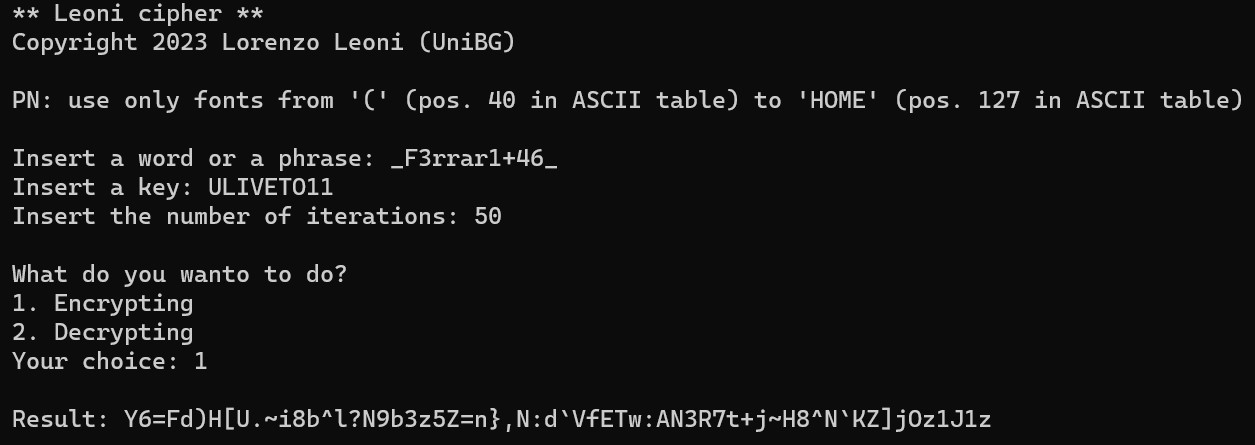
\includegraphics[height=175px]{Immagini/Screenshot1.jpg}}
		\subfigure[]{\label{Screen2}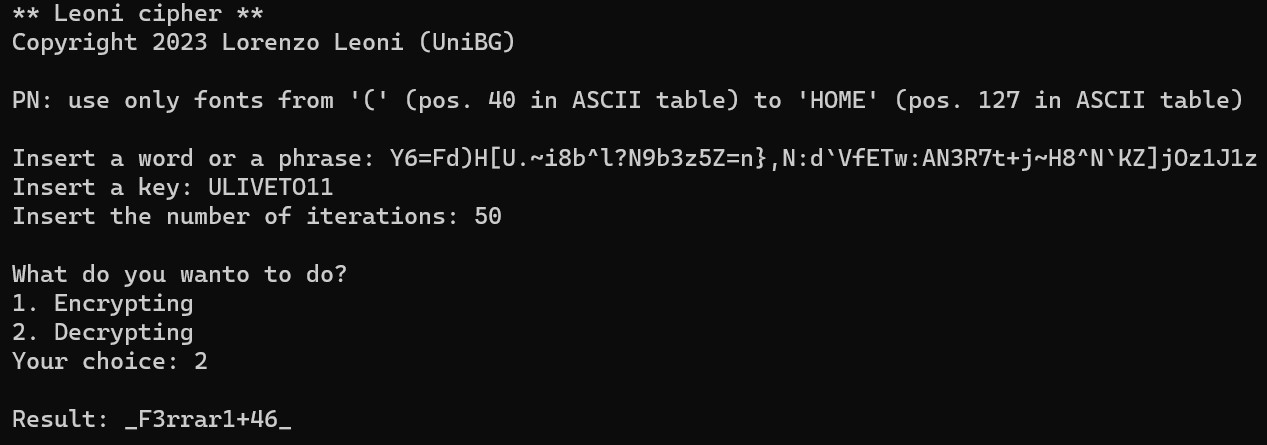
\includegraphics[height=175px]{Immagini/Screenshot2.jpg}}
		\caption[]{un paio di screenshot dell'applicazione in esecuzione.}
		\label{App_screens}
	\end{figure}

\end{document}